\subsection{USB Connection}
Um verschiedene Befehle und den vom Detektor berechneten Winkel vom Android-Phone an das Freedom-Board (KL25Z) 
zu senden, wird eine USB\footnote{Universal Serial Bus}-Schnittstelle zwischen diesen zwei Geräte verwendet.
\newline
Da Android keine native Anbindung an MicroController-Boards via USB zur Verfügung stellt, muss auf 
Frameworks von Drittanbietern zugegriffen werden. In unserem Fall verwenden wir UsbSerial \cite{Inf:UsbSerial} als support-library, wie im Namen ersichtlich, 
handelt es sich dabei um eine virtuelle serielle Schnittstelle (COM-Schnittstelle \footnote{Component Object Model})
für den USB-Port eines Android-Gerätes. Dieser Serial Controller erlaubt es programmatisch alle nötigen Konfigurationen 
(Baudrate, Databit, Stopbits, Paritybit, Flowcontrol) für das Board zu setzen. Mittels einer einzigen 
Methode können nun anschliessend Bytes gesendet werden. Um ein ressourcenfressendes Pollen am Eingang zu vermeiden, 
bietet die Library eine Callback-Funktion, die aufgerufen wird, wenn Daten am Eingang eintreffen.
\newline
Mit dem Programmieren und Erstellen eines ersten Prototyps (Android App, siehe Abbildung \ref{abb:ScreenshotSerialPortExample}) musste die Frage geklärt werden, 
ob mit der support-library das Senden eines einzelnen Strings (Char) zum Freedom-Board und das Echo des 
Boards auf dem Bildschirm des Smartphones ausgegeben werden kann. Nach einem Testlauf zeigte sich, dass
das Senden des Chars soweit nachvollziehbar einwandfrei funktioniert. Beim Empfangen der Daten zeigte 
sich, dass beim parsen der Bytes im Code der support-library ein oder zwei Bits falsch gesetzt wurden. 
Das hatte zur Folge, dass gewisse Buchstaben oder Zahlen nicht mehr korrekt in ASCII 
\footnote{American Standard Code for Information Interchange} respektive UTF-8 
\footnote{Universal Coded Character Set + Transformation Format—8-bit}
umgewandelt werden konnten. Bei einer Handvoll Buchstaben und Zahlen (f, z, o, w, 2-8) funktionierte die
Echo-Methode einwandfrei, bei allen anderen Zeichen jedoch nicht.
\newline
\begin{figure}[h!]
	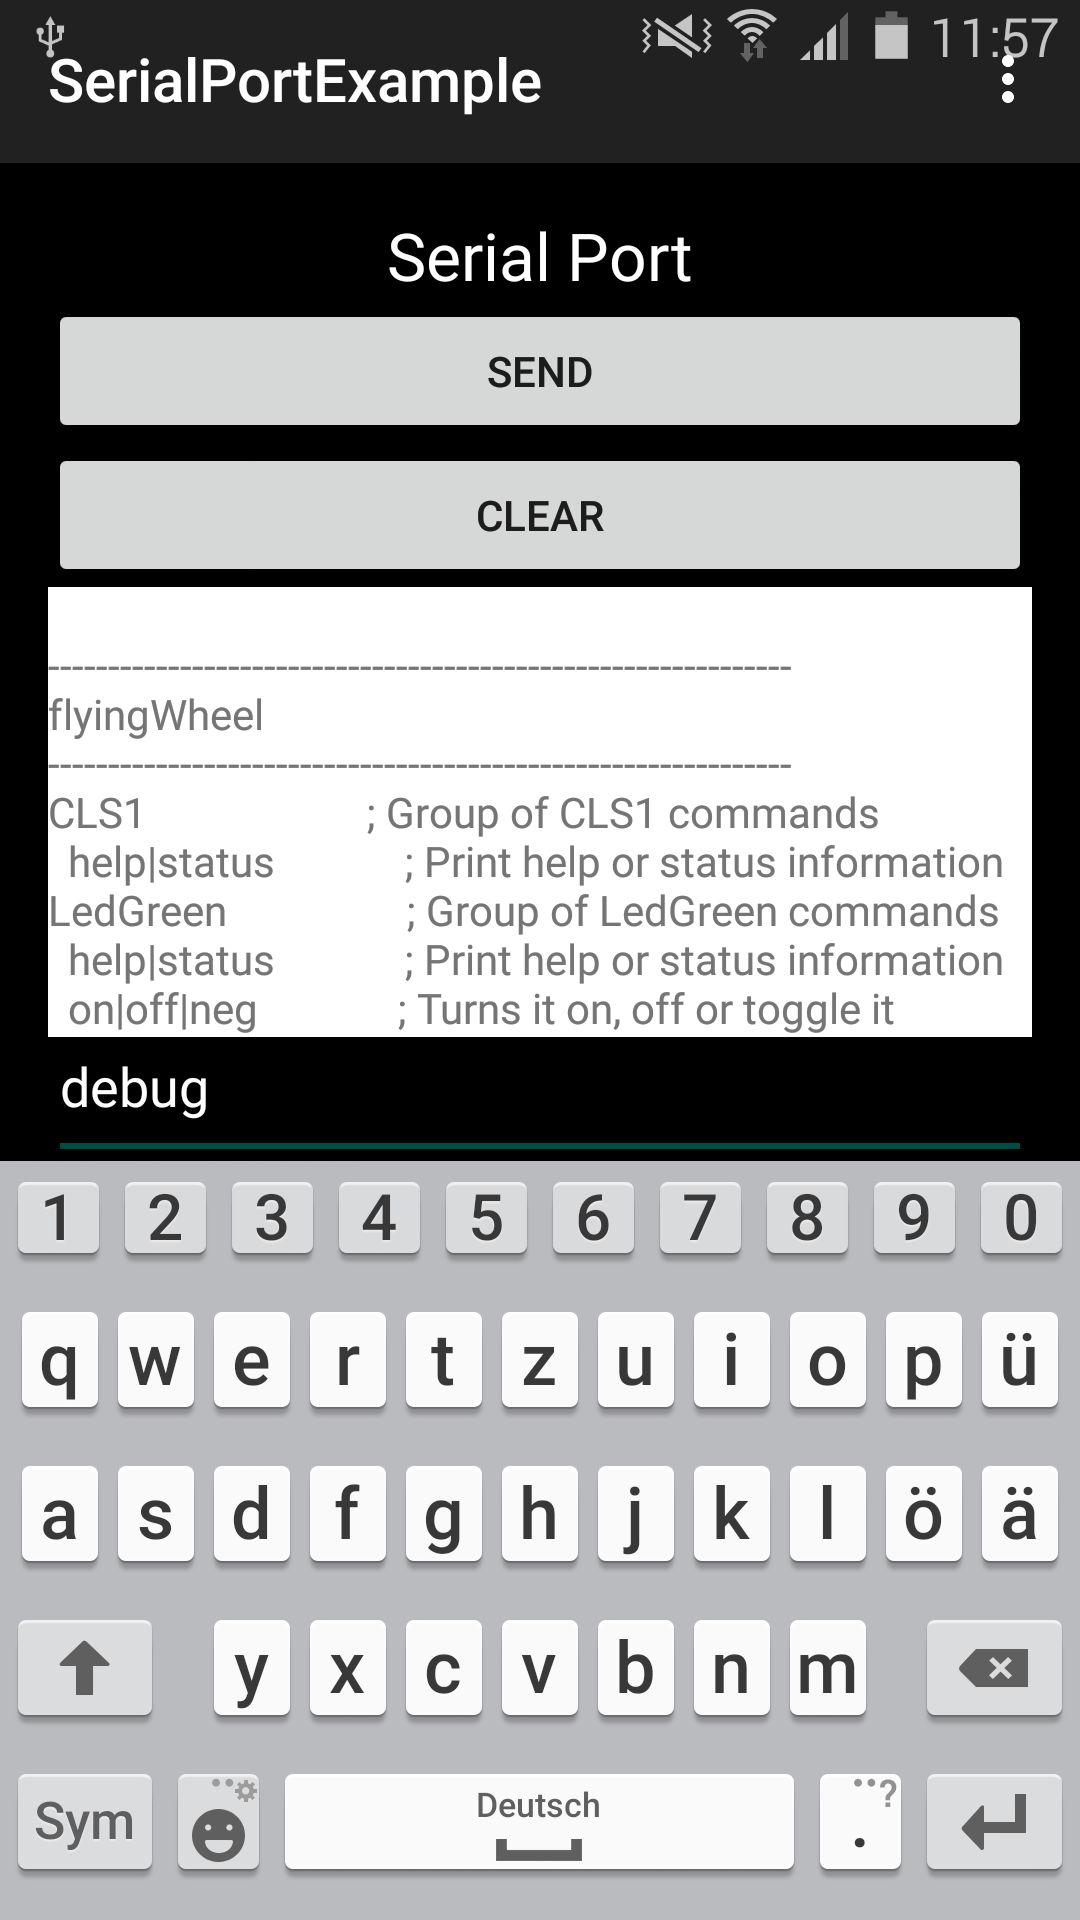
\includegraphics[width=0.3\textwidth,clip,trim=0mm 0mm 0mm 0mm]
	{Enddokumentation/Bilder/Screenshot_SerialPortExample_debug.png}
	\centering
	\caption{Screenshot Prototypen-App zur USB Kommunikation}
	\label{abb:ScreenshotSerialPortExample}
\end{figure}
\newline
Nach einem Update Mitte Februar 2015 durch den Entwickler der support-library funktioniert die App nun 
in bidirektionaler Richtung ohne Einschränkungen. Teil des Updates (respektive einziger Grund) war die 
Erweiterung der unterstützten Geräte um die CH34xSerialDevice-Schnittstelle. Damit erklärt sich auch das 
Fehlverhalten der  App vor dem Update, als die Bits nur bruchstückweise richtig geparst wurden. Es lag 
an der damals schon vorhandenen Schnittstelle zu der CDC-Geräte-Gruppe \footnote{Communication Device Class}, 
die nicht alle Geräte voll, sondern nur teilweise unterstütze und zu einem dieser nicht vollumfänglich 
unterstützen Typen gehörte das Freedom-Board. \newline
Der Code aus dem  Prototyp-App wird nun gewissermassen als Komponente zur Kommunikation mit dem USB-Gerät
im Android-App verwendet. 
\newline
\newline
Die Logik und Auslösung der Befehle an die Motoren findet vom Android-App via Freedom-Board statt. Damit 
sind das Starten der Brushless-DC-Motoren, das Ausrichten des Geräts mit dem Schrittmotor und das Starten 
des Motors für das Förderband gemeint. Nach dem Ausführen ihrer Aufgabe müssen die betreffeden Motoren 
ausgeschaltet werden, das wiederum vom Android-Phone aus passiert.
